\subsection{Deploying Science Pipelines Releases}
\label{sec:scipipe-deploy}

DM has three types of ``release'', each with a different cadence, for
science pipeline related products: \texttt{daily} (also referred to as a \texttt{nightly}), \texttt{weekly}, and \texttt{cycle} or ``major'' release, which have historically occurred once per DM planning cycle (\S\ref{sec:agile}).
A ``major'' release includes a human edited ``changelog'', updated installation
instructions, usage notes, and a formal data processing characterization report,
and thus cannot be completely automated.  However, the
mechanical steps of tagging, building, and publishing software do share
Jenkins pipeline code with the automatically triggered \texttt{daily} and
\texttt{weekly} releases.
The \texttt{daily} and \texttt{weekly} are fully automated and triggered by Jenkins on a fixed
schedule.

\subsubsection{The ``Weekly Release'' pipeline}
\label{sec:releases_weekly}
\label{sec:releases_daily}

The weekly and nightly release pipelines (Fig.~\ref{fig:weekly-pipeline}) are highly similar and
principally differ in that a nightly release does not tag git
repositories.  The rationale is that a nightly is used both for
developer convenience and as a \emph{canary} to ensure that code changes have not
broken the release workflow, but they are not a product that needs to be
reproducible/rebuildable from source.
Both release types share a library of common Jenkins pipeline methods and
will be merged in the near future into a single pipeline script that uses
a separate external configuration per release type.

\begin{figure}[t]
\begin{center}
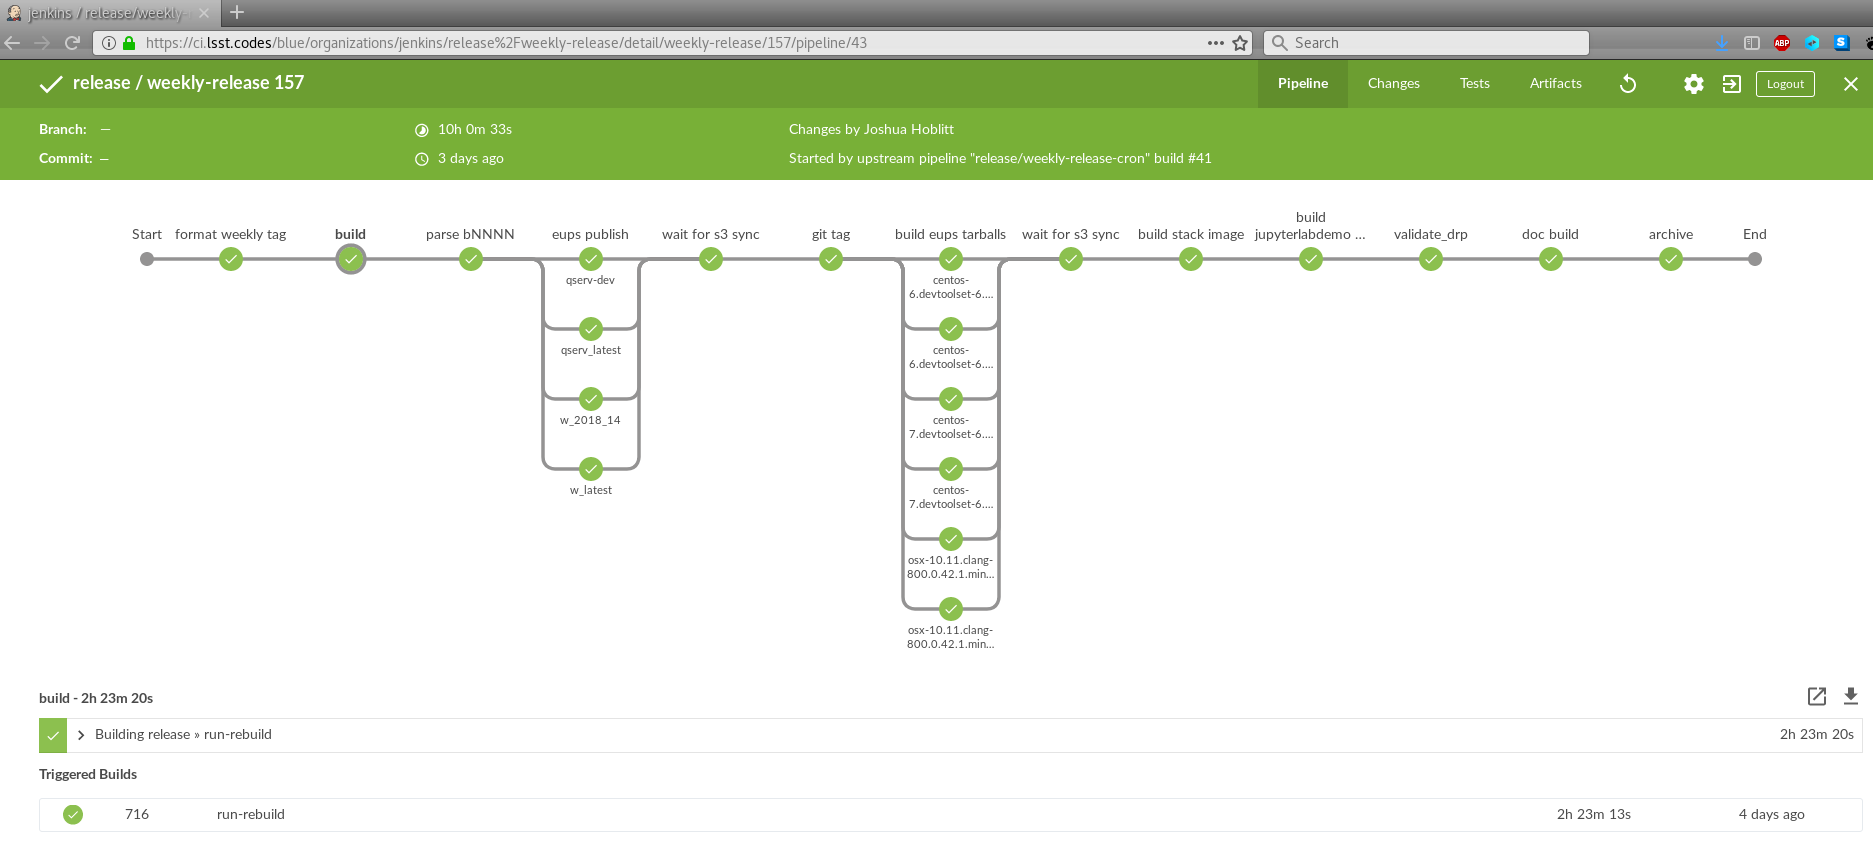
\includegraphics[width=0.7\textwidth]{pipelinedeploy-weekly-release}
\caption{The Jenkins pipeline used for the weekly releases.
\label{fig:weekly-pipeline}}
\end{center}
\end{figure}

\noindent \textbf{``Touchstone'' build \& publish doxygen docs.}
The first step in producing a release is to make a build from the
\texttt{master} branch of the source git repositories on the ``reference''
platform, which is presently \texttt{CentOS~7}.  If the per product unit tests
and a ``quick'' integration test succeed, a cross-package HTML
formatted documentation set is built using \texttt{doxygen}\cite{doxygen} and is published to
a service that developers may access with a web browser.
A ``manifest'' listing the \texttt{eups} products that were part of the build,
git repository SHA1s for those products, and build dependencies are recorded by
\texttt{lsst\_build} at this stage in a git repository structure which the tool
refers to as \texttt{versiondb}.  The canonical ``versiondb'' instance for science
pipeline releases is published on GitHub at
\href{https://github.com/lsst/versiondb}{\texttt{lsst/versiondb}}.

\noindent \textbf{Publish eups source packages.}
\label{sec:scipipe-deploy-src}
\texttt{eups} (\S\ref{sec:eups}) ``source packages'', known as \texttt{eupspkg}, are
produced from the installation tree resulting from the prior step.  Note that
although \texttt{eupspkg} are source-based, and do not contain binary objects,
they require a complete binary installation as input to the packaging process.
In addition to \texttt{eupspkg}, a \texttt{eups} ``distrib tag'' is also
published, which is used to refer to a specific set of packages at fixed
versions.  Examples of \texttt{eups} tags are: \texttt{w\_2018\_14}, \texttt{d\_2018\_04\_10}.

The \texttt{eupspkg} are pushed to an AWS S3 ``bucket'', which is used as the
canonical repository for both source and binary \texttt{eups} packages.  The S3
bucket is not publicly accessible as \texttt{eups} only supports remote
package repositories over \texttt{http[s]} that have HTML ``index
pages'' in the traditional format produced by the \texttt{apache}
webserver.  To accommodate this
requirement, the S3 bucket is periodically replicated to a simple
service that deploys on a Kubernetes cluster providing \url{https://eups.lsst.codes/stack/src/}.

\noindent \textbf{Tag git repos.}
A script contained in the
\href{https://github.com/lsst-sqre/sqre-codekit}{\texttt{sqre-codekit}} package
uses the initial build ``manifest'' to apply an annotated git tag to all
repositories from which an \texttt{eups} product was pulled as part of the
build along with a number of ancillary git repositories that contain build
scripts, documentation, and other items that would be needed to exactly reproduce the
release.
%%WOM above could be shortened

\noindent \textbf{Build/publish eups binary ``tarball'' packages.}
This is perhaps the most complex stage in a release.  Multiple builds/publishes
are run in parallel.  As of the \texttt{15.0} (\texttt{eups} distrib tag
\texttt{v15\_0}) release, the build matrix is: Python 3 on CentOS~6, CentOS~7, and macOS 10.12 (in 10.9 compatibility mode).
We use the GCC\,6 compiler from \texttt{devtoolset-6} on Linux and the Apple \texttt{clang} compiler matching the macOS version.

Every build is started from scratch and bootstraps a development/installation environment using the \href{https://github.com/lsst/lsst/blob/master/scripts/newinstall.sh}{\texttt{new\-install.sh}}\cite{pipelines-guide} script, just as an ``end user'' would when building/installing science pipeline software.

Then a \texttt{eups distrib install} is performed, also as an end-user would
run.  This is followed by publishing \texttt{eups} ``distrib tarballs'' (binary
packages) to a local path.  \texttt{newinstall.sh} is again executed but into a
new path.  The second, pristine, installation is pointed at the local publication
path, rather than the public \texttt{EUPS\_PKGROOT}, and does a complete binary
installation.  This is followed by some simple acceptance tests, such as
building another package from source against the binary installation.  If there
are no failures, the binary ``tarballs'' are then publicly published in a
similar manner to the ``source'' \texttt{eupspkg} but using a different
directory prefix to prevent source and binary packages from different
environments from being intermixed.
%%WOM above could be much shorter.. we install we check we done

\noindent \textbf{Build docker image.}
A \href{https://github.com/lsst-sqre/docker-tarballs}{Docker image} is
constructed with the ``tarballs'' from the release pre-installed, which is
published to Docker hub in the
\href{https://hub.docker.com/r/lsstsqre/centos/}{\texttt{lsstsqre/centos}} repository.

The SCons-based build/installation (\S\ref{sec:sw-packaging}) that is used by all science pipelines software installs
virtually all files from the build tree. This includes \texttt{.o} files, unit
test scripts, test data, and \texttt{doxygen} HTML and XML output. In
addition, none of the executable binaries have been \texttt{strip(1)}d.  This is primarily to assist further development and debugging.  These
excess materials, which are unlikely to be of interest to an end user or in a
production system,
 %would add approximately 6\,GB to an uncompressed Docker image and
%would result in an overall size around 10\,GB.  To avoid frustrating downstream
%consumers, the aforementioned items
are stripped from the Docker layer resulting in an uncompressed image of less than 6~GB.

\noindent \textbf{Build jupyterlab docker image}
The ``release'' docker image is used as the base (\texttt{FROM}) for the
jupyterlabdemo base image (\S\ref{sec:jupyterlab}).  This results in both
``nightly'' and ``weekly'' builds becoming available in a Jupyterlab environment
with relatively low latency.

\noindent \textbf{Process test data sets and collect metrics}
The ``release'' docker image is also used to run several test data sets using a
package called
\href{https://github.com/lsst/validate_drp/}{\texttt{validate\_drp}}.
Metrics are collected from the processing results and are shipped to a
dashboard called ``\href{https://squash.lsst.codes/}{SQuaSH}''\cite{SQR-009}, which plots
trends over time.

\noindent \textbf{Experimental documentation build \& publish}
Due to the ease of ``composition'' with Jenkins pipelines, it is relatively low
cost to add additional pipeline stages on a temporary basis in order to test out
new features.  Presently, this stage is ``tacked on'' to the regular release
workflow in order to evaluate a new documentation build and publish process in parallel
with the existing \texttt{doxygen}-based build.
